\documentclass[border=0cm]{standalone}
\usepackage{tikz}
\usetikzlibrary{calc,intersections,through,backgrounds}

\begin{document}

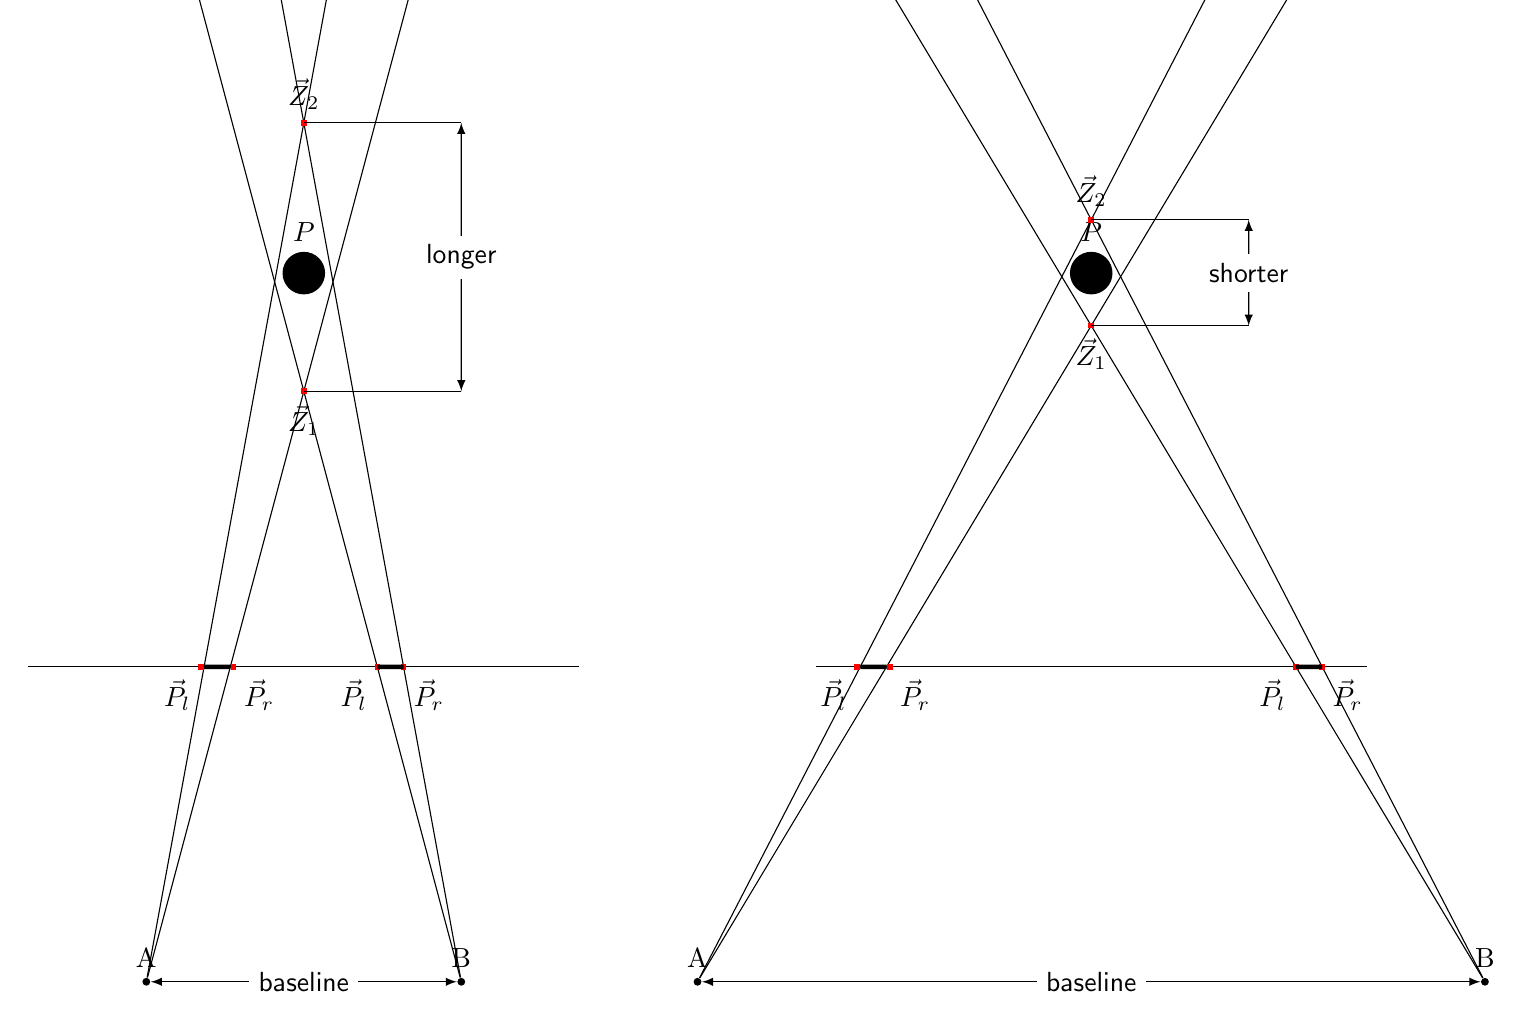
\begin{tikzpicture}[
		dot/.style={circle,inner sep=1pt,fill,label={#1},name=#1},
		dott/.style={name=#1},
		extended line/.style={shorten >=-20cm,shorten <=-0cm},
		dimen/.style={<->,>=latex,thin,every rectangle node/.style={fill=white,midway,font=\sffamily}},
]

\def\worldY{5}
\def\scrY{8}
\def\camY{-4}
\def\pixW{0.5}
\def\guideline{2}
\def\axislen{3.5}
\def\sceneseparation{10}

%\draw (-30, \scrY) -- ++ (60, 0);

\newcommand*{\rendercam}[5]{%
	% #1 = camx
	% #3 = scrx
	\def\camx{#1}
	\def\scrx{#2}
	\node [dot=#5] at (\camx, \camY) {};
	\node [dott=Pl] at (\scrx-\pixW, \scrY) {};
	\node [dott=Pr] at (\scrx+\pixW, \scrY) {};

	\draw [extended line, name path=#3] (#5) -- (Pl);
	\draw [extended line, name path=#4] (#5) -- (Pr);

}

\newcommand*{\scene}[3]{
	%\draw (0, -5) -- ++(0, 20);
	\draw [name path=sensoraxis] (-\axislen, 0) -- (\axislen, 0);
	\node[dot=$P$] at (0, \worldY) {lol};

	\rendercam{-#1}{-#2}{ALl}{ALr}{A}
	\rendercam{#1}{#2}{ARl}{ARr}{B}

	\draw [dimen] (A) -- (B) node {baseline};

	\path [name intersections={of=ALl and ARr}];
	\node [fill=red,inner sep=1pt,label=90:$\vec Z_2$] at (intersection-1) {} coordinate (Za);
	\draw [thin] (intersection-1) -- ++(\guideline, 0) coordinate (Zaa);

	\path [name intersections={of=ARl and ALr}];
	\node [fill=red,inner sep=1pt,label=-90:$\vec Z_1$] at (intersection-1) {} coordinate (Zb);
	\draw [thin] (intersection-1) -- ++(\guideline, 0) coordinate (Zbb);
	\draw [dimen] (Zaa) -- (Zbb) node {#3};

	\path [name intersections={of=ALl and sensoraxis,name=uuh}];
	\path [name intersections={of=ALr and sensoraxis,name=aah}];
	\node [fill=red,inner sep=1pt,label=-100:$\vec P_l$,left] at (uuh-1) {};
	\node [fill=red,inner sep=1pt,label=-80:$\vec P_r$,right,right] at (aah-1) {};
	\draw [ultra thick] (uuh-1) -- (aah-1);

	\path [name intersections={of=ARl and sensoraxis,name=uuh}];
	\path [name intersections={of=ARr and sensoraxis,name=aah}];
	\node [fill=red,inner sep=1pt,label=-100:$\vec P_l$] at (uuh-1) {};
	\node [fill=red,inner sep=1pt,label=-80:$\vec P_r$] at (aah-1) {};
	\draw [ultra thick] (uuh-1) -- (aah-1);

}

\scene{2}{-0.7}{longer}

\begin{scope}[xshift = \sceneseparation cm]
	\scene{5}{-1.7}{shorter}
\end{scope}

\end{tikzpicture}
\end{document}
